% REMEMBER: You must not plagiarise anything in your report. Be extremely careful.

\documentclass{l4proj}

    
%
% put any additional packages here
%

\begin{document}

%==============================================================================
%% METADATA
\title{This will be the title one day}
\author{Paul Bekaert}
\date{September 14, 2018}

\maketitle

%==============================================================================
%% ABSTRACT
\begin{abstract}
    Every abstract follows a similar pattern. Motivate; set aims; describe work; explain results.
    \vskip 0.5em
    ``XYZ is bad. This project investigated ABC to determine if it was better. 
    ABC used XXX and YYY to implement ZZZ. This is particularly interesting as XXX and YYY have
    never been used together. It was found that  
    ABC was 20\% better than XYZ, though it caused rabies in half of subjects.''
\end{abstract}

%==============================================================================

% EDUCATION REUSE CONSENT FORM
% If you consent to your project being shown to future students for educational purposes
% then insert your name and the date below to  sign the education use form that appears in the front of the document. 
% You must explicitly give consent if you wish to do so.
% If you sign, your project may be included in the Hall of Fame if it scores particularly highly.
%
% Please note that you are under no obligation to sign 
% this declaration, but doing so would help future students.
%
\def\consentname {Paul Bekaert} % your full name
\def\consentdate {7 October 2022} % the date you agree
%
\educationalconsent


%==============================================================================
\tableofcontents

%==============================================================================
%% Notes on formatting
%==============================================================================
% The first page, abstract and table of contents are numbered using Roman numerals and are not
% included in the page count. 
%
% From now on pages are numbered
% using Arabic numerals. Therefore, immediately after the first call to \chapter we need the call
% \pagenumbering{arabic} and this should be called once only in the document. 
%
% Do not alter the bibliography style.
%
% The first Chapter should then be on page 1. You are allowed 40 pages for a 40 credit project and 30 pages for a 
% 20 credit report. This includes everything numbered in Arabic numerals (excluding front matter) up
% to but excluding the appendices and bibliography.
%
% You must not alter text size (it is currently 10pt) or alter margins or spacing.
%
%
%==================================================================================================================================
%
% IMPORTANT
% The chapter headings here are **suggestions**. You don't have to follow this model if
% it doesn't fit your project. Every project should have an introduction and conclusion,
% however. 
%
%==================================================================================================================================
\chapter{Introduction}

% reset page numbering. Don't remove this!
\pagenumbering{arabic} 

\section{Motivation}

The game of life has often been seen as a toy project. It is idealistic in its representation, as it is fully observable, episodic and deterministic. However, its simple rules give rise to complex structures that are not easy to find. Those structures can be large, and looking for them is unfeasible with the current methods. In general, conventional graph search methods adapted to the task are are used, but they are slow and require large amounts of memory \cite{list_of_search_algorithms}, and as mentioned, they cannot find objects that are too large. There is, as of yet, no efficient way to search for these structures, and the question remains if there is a way to do it.

The concept of using deep learning to find structures in cellular automata has not yet been explored. With the advent and rise of neural networks, previously thought to be impossible problems have been unlocked, either by solving them directly or speeding up existing search algorithms. Since this is a difficult search problem, it stands to reason that solving it will potentially give new insights into how to solve similar problems.

\section{Aims}

In this paper, we will be trying to find interesting structures in the game of life. Our particular interest will be in oscillating objects that move a set amount of space, so-called 'Spaceships'. The main goal will be to test and see if neural networks can speed up the search, and how different deep learning techniques fare against each other and other conventional search methods. The expectation is that the network will greatly decrease the time it takes to find novel structures or structures already classified as spaceships.

[MAYBE TALK ABOUT AIMS WITH GOL AND DEEP LEARNING]


%==================================================================================================================================
\chapter{Background}

\section{The game of life}
% ========

\subsection{Rules}

"The Game of Life" is a zero-player game invented by John Conway in 1970 which describes a cellular automata (CA) with a set of rules. A cellular automata is a board is made out of a grid size $n\times m$ , with each square being a cell. A cell is either dead or alive, represented as a $1$ or a $0$ respectively. The rules of the game can be defined in different ways, but the one John Conway proposed is the most well known. The neighbourhood of the cell is defined as Moore's neighbourhood, which is the 8 cells adjacent to the cell, diagonally and orthogonally. It can also be thought of as a $3\times 3$ matrix where the subject cell is placed in the middle. The number of neighbours the cell has is the number of cells alive that are present in the cell's Moore neighbourhood, $n$. We can then define the rules of the CA described in Life:

\begin{itemize}
    \item A dead cell turns into a living cell if $n \geq 3$
    \item A dead cell stays dead if $n < 3$
    \item A living cell stays alive if $n = 2$ or $n = 3$
    \item A living cell dies if $n < 2$, due to under-population
    \item A living cell dies if $n > 3$, due to overcrowding
\end{itemize}

A state at $t+1$ is entirely dependant on the current state at $t$ and is calculated using the rules above.

\begin{figure}[h]

\begin{subfigure}{0.5\textwidth}
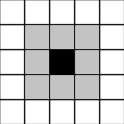
\includegraphics[width=0.9\linewidth, height=6cm]{dissertation/images/moores_law.png} 
\caption{Moore's Neighbourhood}
\label{fig:subim1}
\end{subfigure}

\caption{Examples of Moore's neighbourhood}
\label{fig:image2}
\end{figure}

\subsection{Still lifes}

A still life is a structure that does not move or change shape from generation to generation. They remain static, unless outside cells interact with it. Still lifes are by far the most known structures in the GoL, and they are easy to find, as they have the same shape for $t$ and $t+1$. Here are some examples of still lifes:

\subsection{Oscillators}

These are structures that change shape, but return to the same state every $p$ generations. They are a little harder to detect, as it is impossible to know how many generations it will take for the structure to repeat. An oscillator will stay in the same position after it has oscillated, and will keep oscillating as long as it is undisturbed by other cells and the program keeps running. Here are some examples of oscillators:

\subsection{Spaceships}

Spaceships are the main focus of this paper, and are the hardest structures to detect. They are similar to oscillators in that they repeat their state every $p$ generations. However, they also move a certain distance since their last oscillation. If the state space they are in is unbounded, then they will move forever without changing direction.

The speed of a spaceship is determined in terms of the speed of light of GoL, $c$. This $c$ is defined as 1 cell per second, as it is theoretically the quickest information could hope to propagate given the rules of Life. The ship can move diagonally, orthogonally, or knightwise, which is when a ship moves in an oblique direction. A spaceship with a period $p$, which is moving $n$ cells in a particular direction is said to have a speed $nc/p$. A ship moving $n = 2$ cells left and with a period $p = 5$ will have a speed of $2c/5$. For a ship moving knightwise $n$ cells either left or right, and $m$ cells either up or down, will have a speed denoted as $(m, n)c/p$. These speeds can be simplified, for example a spaceship moving at speed $2c/4$ can be written as $c/2$.

A further way to classify spaceships is by their type. 
% should you explain this?

Examples of spaceships [ADD MORE EXAMPLES]:

\begin{figure}[h]
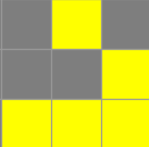
\includegraphics[width=0.9\linewidth, height=6cm]{dissertation/images/glider.png} 
\caption{The glider}
\label{fig:subim1}
\end{figure}

% ========
\section{Existing Search Methods}

There are not many papers on the subject, but one notable paper is "Searching for Spaceships" \cite{searching_for_spaceships}, which uses an algorithm "gfind", using a mix of breadth first search and depth first iterative deepening. The search takes place row-by-row, and uses a pre-calculated hash table of cell configurations to remove impossible rows from the search, narrowing down the graph. This method only works for small periods, as larger ones run out of memory quite quickly. It also only finds orthogonal spaceships, and they must be symmetrical along one of its axis. It was used to find some common spaceships, and did improve on speed, but did have its limitations.

Another well known algorithm to find spaceships or oscillators is "lifesrc" created by David Bell, uses a depth first backtracking search. The grid is first set up with a few 'known' cells, set by the user. The rest of the cells are classed as 'unknown'. When the algorithm starts running, a decision is made on whether a cell should be alive or not, and the program will check forward and backward if there are any oscillating patterns of period $p$ set by the user. If nothing is found, the search continues, using the decided cell. If it is found later on that a cell placement in a particular cell is impossible, or that there are no oscillators in a particular configuration, then the algorithm will backtrack to the latest cell it decided on randomly. This is essentially a depth first search, however it discards certain sub-trees by eliminating ones that do not follow the Life rules (for example, checking if every cell is alive in a $4 \times 4$ grid would be redundant, since almost all cells in that grid would die in the next iteration). 

The most efficient algorithm used to find spaceships today is dubbed the 'ikpx2' algorithm, which was created by Adam P. Goucher. It was inspired by gfind, which searches De Bruijn graphs representing the different parts of a spaceship. However, ikpx reduces the spaceship search problem into a set of SAT constraints, which can then be used on an SAT solver. The solver used in question is the "iglucose" \cite{sat_2018} SAT solver and sped up the search considerably, as a lot of research has gone into accelerating SAT solvers. A notable find by the ikpx2 algorith was the 'knightship': the first oblique spaceship found, or in other words, a spaceships that does not move diagonally nor orthogonally.

\section{Deep Learning with the GoL in General}

There are a few research papers written on neural networks and the game of life, with one notable one being about forward planning in the GoL \cite{game_of_life_dl_is_hard}. In this paper, they try to predict the future structure of a starting configuration. They used several 1x1 and 3x3 convolutional layers in their network, activated by ReLU functions. Although the model was able to perfectly predict the next iteration of the game, the further the model tries to predict, the worse the result. The problem hypothesised by Springer is the 'lottery ticket problem', in which the starting configuration of the model is what would allow it to converge to a correct solution. [MAKE SURE THIS IS CORRECT AND REPHRASE]

Apart from research done, there are many hobbyists working on combining deep learning with GoL. One of them is James McGuigan, who trained a neural network to learn the game of life after one iteration. He has also worked on reversing the game of life, trying to find a previous configuration using a current board state. Another notable use of deep learning and the game of life is by NeatAI, who used genetic algorithms in the game of life \cite{neatai_gol}. He used a $c$ function that calculates the overall 'complexity' of the current structures in the grid. For example, a grid with random cells is not very interesting, but one that has a couple of gliders and oscillators with high periods may be of more interest. To design his $c£$ function, he took inspiration from a paper by \cite{algorithmic_specified_complexity}, which describes a process of encoding interesting objects in the game of life. It uses features of an object such as shift, repeating period, intersection between 2 or more objects, to define the properties of such an object, These properties are then bit-encoded to form a number that specifies the complexity of the object. To find the complexity of a particular state on a board, the sum of the object complexities is taken.

NeatAI took this $c$ function and applied it to a neural network which determined whether or not a cell should be alive given the input parameters $x$, $y$, population density, and bias. He then used genetic neural networks to improve his model to maximize the $c$ function. The net improved by making optimal start configurations for the model to evolve into. This is an interesting concept, as if the $c$ function were to be changed to be maximised by how far a pattern has reached from the origin, it could potentially be used to find new spaceships for example.

%==================================================================================================================================

\chapter{Analysis}

\section{Different ways to find spaceships}

The problem we're trying to solve is to find spaceships. These are, as explained above, structures that repeat inside of a game of life grid, but also move a certain amount of space. This is a widely known toy problem, however it is an NP-hard problem, which means brute force is out of the question. In a given $n \times m$ grid, there are $2^{n \times m}$ possible combinations. For example, a glider, which takes at least a $3x3$ grid to be represented, would be found by searching $2^{9}$ grids. Brute force becomes unfeasible after approximately $n > 6, m > 6$. This algorithm tends not to have much use, but it has found a comprehensive list of all still-lives, oscillators, and spaceships within a small rectangle.

A better approach is representing the board as a graph. By representing each cell as a path- a path where the cell is either alive or a path where the cell is dead- a tree search method can be used. This is the method used in most algorithms today, by trying to optimize which cell should be placed next. Some combinations of cells should not be placed together as the result would be incompatible with a spaceship, and therefore the algorithm can eliminate entire sub-trees from the search space.

In Searching for Spaceships \cite{searching_for_spaceships}, a de Bruijn graph is used to represent the cells. The algorithm only works on one side of the ship, and assumes the other to be symmetrical. A ship is then constructed by applying the GoL rules to rows of the ship, and placing the formed cell in front of the ship in the direction it will move. To visualize this, imagine the grid follows the ship as it is moving, so that the ship looks like it is simply oscillating. A future oscillation can therefore be predicted by taking the evolution of the spaceship for every row of 3, and applying it $p$ (the speed of the ship) cells above the evolution, as it would reach that point p next iteration. This approach has one major drawback- any spaceship that is not a "long" spaceship will not be detected. The search space also does not include non-symmetrical spaceships, of which there are many.

% should this be in the background section?
\section{Similar Problems and how they are Solved}

MAYBE TALK ABOUT CHESS OR SOMETHING HERE

\section{The Main Assumption}
Neural networks are good at detecting general patterns which can be hard to detect as humans. There has been a lot of debate in the GoL community about an underlying pattern to spaceships. There have been methods by the community which use "spaceship engineering" - combining multiple identified sub-parts of spaceships to make a new moving ship. However, there has yet to be a formalized equation or pattern found to help fast-track the search of such ships. To use a neural network for this problem, the approach taken in this paper revolves around the assumption that spaceships have an underlying pattern which is detectable to a neural network. Although there are not many spaceships, data expansion methods are used to gather more data, and convolutional techniques are used to train the network.
% maybe add stuff about the scoring algorithm here?

\section{The Solution in this Paper}


%==================================================================================================================================
\chapter{Design}
How is this problem to be approached, without reference to specific implementation details? 

\section{The Networks}
There are two main networks that this algorithm will use to guide the search:
\begin{itemize}
    \item The probability network: used to find which cells should be modified
    \item The scoring network: used as a heuristic function
\end{itemize}
The probability network uses a fully convolutional network without pooling layers. The network follows two $3 \times 3$ convolutions, with out channels of 3 and 12. This is followed by a $1 \times 1$ convolution with an out channel of 24, and finally two $5 \times 5$ layers with out channels 48 and 96. The final convolution is a dimensional reduction, reducing the out channels to 1. Each convolutional layer except the last uses a swish activation function/ Additionally, padding is used to keep the input size the same as the output size.

The network takes as input a configuration of cells with values ranging from 0 to 1. The 

- talk about the scoring network

\section{Data used to train the network}
- What spaceship sizes used
- Expansion of the data
- Deconstruction of data
- Modifying data to predict the change in probability
- Scoring data and random configuration


\section{The Algorithm}

- talk about joining everything together

The algorithm is a standard tree search, but uses two neural networks to help accelerate it. The first network is trained to predict the probability change that a cell should be present given a structure. This will then be used in a tree search algorithm, with branches generated given the highest changes in probability. The second network is trained to predict the mean square error of a given configuration. This is to be used as a heuristic for the A* algorithm.

The probability prediction network receives as input a grid of arbitrary size with probability values between 0 and 1. The network will then predict a change in probability grid. The highest changes in probability (positive or negative) are then applied to a new grid. these grids then become the branches of a node. Using the scoring network, the grid with the lowest score is then chosen to be the next node. This is effectively an A* search technique.


%==================================================================================================================================
\chapter{Implementation}

ALSO TALK ABOUT PROTOTYPES AND WHY THEY DIDN'T WORK, A PAGE FOR ALL OF THE FAILED ATTEMPTS COMBINED

TALK ABOUT HOW TO IMPLEMENT THE DESIGN: PYTORCH, PIPELINE, ETC (15-18 pages, bulk of the report)

2 main approaches tried:
- Trying to determine a spaceship or not
    - and hence, switching a cell will tell you if it improves the probability of the grid being a spaceship or not
    - This did not work, as a change in 1 cell was not enough to train
    - Training networks tried includes: Using a CNN, 100x100 static, removing n cells and training the network, showing spaceships compared to random data.
- Using a probability grid to determine the most probable cells to place now 
    - Training method: used a CNN with the same output as input. 
    - The model will take an input of cell probabilities, and output a change of probabilties.
    - Different datasets trained on: full 1s with solution being what cells to remove, full 0s with solution being spaceship itself, random noise with solution being change to make it into spaceship, and deconstructing the ship cell by cell and training on every iteration.

\section{General points}
These points apply to the whole dissertation, not just this chapter.


\section{Software Engineering Practices}

- calendar tracking
- waterfall
- github repo
- weights and biases
To keep up with all the work, I logged the hours. I also used a waterfall development technique, where I completed the work one step at a time. 


\section {Unsuccessful Attempts}

\subsection{Ship Likelihood}
My first try to solve this problem revolved over giving structures a "score" as to how close they are to being a spaceship. The idea was that if I could teach a network what is a ship or not, and it could output the likelihood of the structure being a spaceship. 

I used several convolutions and pooling, followed by a adaptive convolutional layer which I then fed to a fully connected network. This would then produce a probability of the structure being a spaceship.

I hypothesise this technique did not work for several reasons: The pooling lost information about the structure, the fully connected network was not able to properly converge, and the output was a softmax which was unreliable. Furthermore, the ships were compared with noisy data. Ships often had a lot of whitespace around them which made them easy to identify, and no solid features could be used.

I fed this neural network to a tree search which worked by flipping cells off and on and checking if the probability of the structure being a spaceship increased. This did not work very well, already because the network did not produce good results, but also because the fully connected layer meant that changing a single cell did not change the final output much.

\section{Challenges faced}

TALK ABOUT HOW YOU TRIED DIFFERENT APPROACHES OF WORKING, THE SIZE OF THE NETWORK AND HOW YOU HAD TO RUN IT ON A DIFFERENT COMPUTER, AND GENERAL FUCKERY THAT HAPPENED DURING THE PROJECT

\section{Probability Search}

\subsection{Choice of Technologies}

Since the idea of the project was to use neural networks to accelerate spaceship search, I needed something like Pytorch for the deep learning.
- Pytorch
- github?
- matplotlib?
- numpy/pandas??
,

\subsection{Architecture of the network}

The implementation which gave me the most results was as mentioned above, several convolutions (without a pooling layer), and a fully connected network for the probability score. This was done using PyTorch. The layers consisted of [MAKE A DIAGRAM OUT OF THIS]:
\begin{itemize}
  \item A first convolution with a 3x3 matrix using a swift activation function
  \item A second convolution with a 3x3 matrix using a swift activation function
  \item A third convolution with a 3x3 matrix using a swift activation function
  \item A fourth convolution with a 3x3 matrix using a swift activation function
  \item A final convolution merging the kernels into one (grid probability output here)
  \item An adaptive pooling of this probability grid into a 100 x 100 tensor 
  \item A fully connected 100 x 100 layer that took the output of the pooling to a 100 tensor layer, using a relu function
  \item Lastly, a linear layer which outputted the 'score' of the prediction
\end{itemize}


\subsection{Graph search}

The graph search was relatively simple and is based off of A*. The search starts with a few "set" cells. This initial grid is fed to the model. The model then returns a probability grid with the change of probabilities. The top change in probabilities are taken, and the cell values are switched. All these swtiched cells are put through the model again, and the 



%==================================================================================================================================
\chapter{Evaluation} 
How good is your solution? How well did you solve the general problem, and what evidence do you have to support that?

        Answer them with precise evidence (graphs, numbers, statistical
        analysis, qualitative analysis).
        Used an average improvement of the different cells, ie, cells that were supposed to be there should have a higher probabiltiy score change; those that were not supposed to be there should have a small change in score (negative), etc. Graphed this for number of iterations along with the number of cells removed and such.
        I also tested the scoring algorithm, to see if it can model the loss function correctly.
\section{Guidance}
\begin{itemize}
    \item
        Ask specific questions that address the general problem.
    \item
    \item
        Be fair and be scientific.
    \item
        The key thing is to show that you know how to evaluate your work, not
        that your work is the most amazing product ever.
\end{itemize}

\section{Evidence}
Make sure you present your evidence well. Use appropriate visualisations, reporting techniques and statistical analysis, as appropriate.

If you visualise, follow the basic rules, as illustrated in Figure \ref{fig:boxplot}:
\begin{itemize}
\item Label everything correctly (axis, title, units).
\item Caption thoroughly.
\item Reference in text.
\item \textbf{Include appropriate display of uncertainty (e.g. error bars, Box plot)}
\item Minimize clutter.
\end{itemize}

See the file \texttt{guide\_to\_visualising.pdf} for further information and guidance.

\begin{figure}
    \centering
    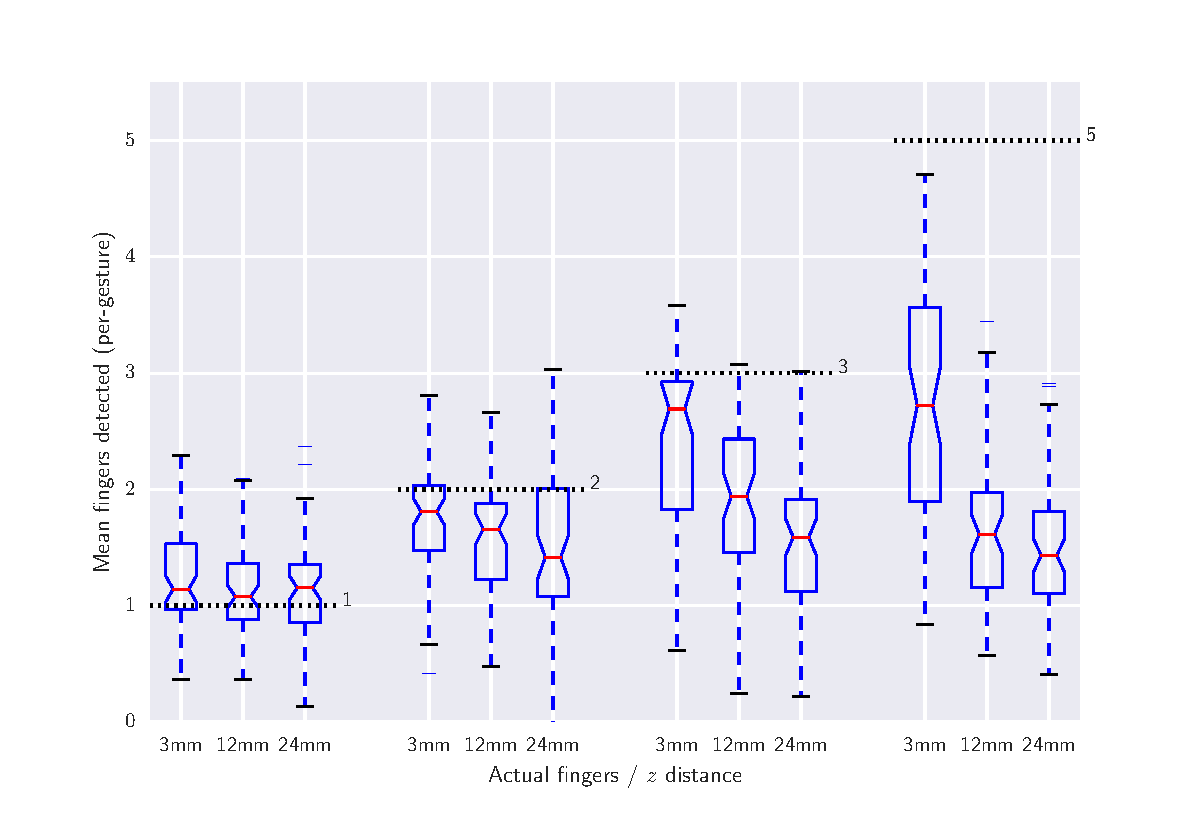
\includegraphics[width=1.0\linewidth]{images/boxplot_finger_distance.pdf}    

    \caption{Average number of fingers detected by the touch sensor at different heights above the surface, averaged over all gestures. Dashed lines indicate
    the true number of fingers present. The Box plots include bootstrapped uncertainty notches for the median. It is clear that the device is biased toward 
    undercounting fingers, particularly at higher $z$ distances.
    }

    % use the notation fig:name to cross reference a figure
    \label{fig:boxplot} 
\end{figure}


%==================================================================================================================================
\chapter{Conclusion}    
Summarise the whole project for a lazy reader who didn't read the rest (e.g. a prize-awarding committee).
\section{Guidance}
\begin{itemize}
    \item
        Summarise briefly and fairly.
    \item
        You should be addressing the general problem you introduced in the
        Introduction.        
    \item
        Include summary of concrete results (``the new compiler ran 2x
        faster'')
    \item
        Indicate what future work could be done, but remember: \textbf{you
        won't get credit for things you haven't done}.
\end{itemize}

%==================================================================================================================================
%
% 
%==================================================================================================================================
%  APPENDICES  

\begin{appendices}

\chapter{Appendices}

Typical inclusions in the appendices are:

\begin{itemize}
\item
  Copies of ethics approvals (required if obtained)
\item
  Copies of questionnaires etc. used to gather data from subjects.
\item
  Extensive tables or figures that are too bulky to fit in the main body of
  the report, particularly ones that are repetitive and summarised in the body.

\item Outline of the source code (e.g. directory structure), or other architecture documentation like class diagrams.

\item User manuals, and any guides to starting/running the software.

\end{itemize}

\textbf{Don't include your source code in the appendices}. It will be
submitted separately.

\end{appendices}

%==================================================================================================================================
%   BIBLIOGRAPHY   

% The bibliography style is abbrvnat
% The bibliography always appears last, after the appendices.

\bibliographystyle{abbrvnat}

\bibliography{l4proj}

\end{document}
